%% abtex2-modelo-trabalho-academico.tex, v<VERSION> laurocesar
%% Copyright 2012-<COPYRIGHT_YEAR> by abnTeX2 group at http://www.abntex.net.br/ 

\documentclass[
	% -- opções da classe memoir --
	12pt,				% tamanho da fonte
	oneside,			% para impressão mudar para twoside para facilitar impressaõ de frente e verso 
	a4paper,			% tamanho do papel. 
	chapter=TITLE,
	sumario=tradicional,
	% -- opções do pacote babel --
	english,			% idioma adicional para hifenização
	brazil				% o último idioma é o principal do documento
]{abntex2}

% ----------------------------------------------------------
% IMPORTAÇÃO DE PACOTES
% ----------------------------------------------------------
\usepackage{helvet}
\renewcommand{\familydefault}{\sfdefault}			% Usa a fonte Arial			
\usepackage[T1]{fontenc}		% Selecao de codigos de fonte.
\usepackage[utf8]{inputenc}		% Codificacao do documento (conversão automática dos acentos)
\usepackage{indentfirst}		% Indenta o primeiro parágrafo de cada seção.
\usepackage{color}				% Controle das cores
\usepackage{graphicx}			% Inclusão de gráficos
\usepackage{microtype} 			% para melhorias de justificação
\usepackage{hyperref}
\usepackage{times}

\usepackage{amsmath}
\usepackage{amsthm,amsfonts}

\usepackage{lipsum}				% para geração de dummy text
\usepackage{import}
\usepackage{blindtext}
\usepackage{soul}
\usepackage{lscape}

\usepackage{algpseudocode}
\usepackage{algorithm}
\algnewcommand{\LineComment}[1]{\State \(\triangleright\) #1}
\makeatletter
\renewcommand{\ALG@name}{Algoritmo}
\makeatother

\graphicspath{ {../images/} }

% ---
% Pacotes de citações
% ---
\usepackage[alf]{abntex2cite}	% Citações padrão ABNT

% ----------------------------------------------------------
% CONFIGURAÇÕES DO PDF
% ----------------------------------------------------------

% alterando o aspecto da cor azul
\definecolor{blue}{RGB}{41,5,195}
\definecolor{black}{RGB}{0,0,0}

% informações do PDF
\makeatletter
\hypersetup{
     	%pagebackref=true,
		pdftitle={\@title}, 
		pdfauthor={\@author},
    	pdfsubject={\imprimirpreambulo},
	    pdfcreator={LaTeX with abnTeX2},
		pdfkeywords={abnt}{latex}{abntex}{abntex2}{trabalho acadêmico}, 
		colorlinks=true,       		% false: boxed links; true: colored links
    	linkcolor=black,          	% color of internal links
    	citecolor=black,        		% color of links to bibliography
    	filecolor=black,      		% color of file links
		urlcolor=black,
		bookmarksdepth=4
}
\makeatother

\setlrmarginsandblock{3cm}{2cm}{*}
\setulmarginsandblock{3cm}{2cm}{*}
\checkandfixthelayout

% --- 

% ----------------------------------------------------------
% FIGURAS E TABELAS
% ----------------------------------------------------------

% ---
% Posiciona figuras e tabelas no topo da página quando adicionadas sozinhas
% em um página em branco. Ver https://github.com/abntex/abntex2/issues/170
\makeatletter
\setlength{\@fptop}{5pt} % Set distance from top of page to first float
\makeatother
% ---

% ----------------------------------------------------------
% ESPAÇAMENTOS
% ----------------------------------------------------------

% O tamanho do parágrafo é dado por:
\setlength{\parindent}{1.25cm}

% % Controle do espaçamento entre um parágrafo e outro:
\setlength{\parskip}{0.2cm} 

\setlength{\ABNTEXcitacaorecuo}{4cm}

% Espaçamento entre headers e texto abaixo
\setlength\afterchapskip{0.2cm}
\setlength\aftersecskip{0.2cm} %espaçamento entre seção e texto
\setlength\aftersubsecskip{0.2cm} %espaçamento entre subseção e texto

% ----------------------------------------------------------
% CORREÇÕES DE ESTILO
% ----------------------------------------------------------

% Estilos das legendos
\captionnamefont{\ABNTEXfontereduzida}
\captiontitlefont{\ABNTEXfontereduzida}
\setlength{\belowcaptionskip}{1pt} % espaçamento depois do título das tabelas/figuras
\setlength{\abovecaptionskip}{1pt} % espaçamento antes da legenda de tabelas/figuras

% Estilos dos títulos

\renewcommand{\ABNTEXchapterfontsize}{\bfseries\normalsize}
\renewcommand{\ABNTEXsectionfontsize}{\itshape\normalsize}
\renewcommand{\ABNTEXsubsectionfontsize}{\normalfont\normalsize}
\renewcommand{\ABNTEXsubsubsectionfontsize}{\normalfont\normalsize}

\renewcommand{\chaptitlefont}{\normalfont\bfseries}
\setsecheadstyle{\normalfont\itshape}
\setsubsecheadstyle{\normalfont}
\setsubsubsecheadstyle{\normalfont}

\renewcommand{\ABNTEXchapterfont}{\bfseries}
\renewcommand{\ABNTEXchapterfontsize}{\normalsize}
\setboolean{ABNTEXupperchapter}{true}

% Estilos nos sumários
\renewcommand{\cftchapterfont}{\MakeUppercase}
\setboolean{ABNTEXupperchapter}{true}

\renewcommand{\cftsectionfont}{\normalfont}
\renewcommand{\cftsubsectionfont}{\normalfont}
\renewcommand{\cftsubsubsectionfont}{\normalfont}

% ----------------------------------------------------------
% COMPILA O ÍNDICE
% ----------------------------------------------------------
\makeindex

% ----------------------------------------------------------
% COMANDOS CUSTOMIZADOS
% ----------------------------------------------------------
\newcommand{\un}[1]{\;\text{#1}}
\newcommand{\logo}{\quad \Rightarrow \quad}
\newcommand{\codeword}[1]{\texttt{\textcolor{black}{#1}}}
\newcommand{\specialcell}[2][c]{%
  \begin{tabular}[#1]{@{}c@{}}#2\end{tabular}}

% ----------------------------------------------------------
% INÍCIO DO DOCUMENTO
% ----------------------------------------------------------
\begin{document}

%\selectlanguage{english}
\selectlanguage{brazil}

% Retira espaço extra obsoleto entre as frases.
\frenchspacing 

% ----------------------------------------------------------
% ELEMENTOS PRÉ-TEXTUAIS
% ----------------------------------------------------------
\import{../elementos-pre-textuais}{capa.tex}
\import{../elementos-pre-textuais}{sumario.tex}

% % ----------------------------------------------------------
% % ELEMENTOS TEXTUAIS
% % ----------------------------------------------------------
\textual

\pagestyle{simple}

\chapter{Modelagem Multiobjetivo}\label{cap:modelagem} 

No TC01, modelamos duas funções objetivo:

\begin{itemize}
	\item $f_1 (\cdot)$: minimização do custo de manutenção total 
	\item $f_2 (\cdot)$: minimização do custo esperado de falha total
\end{itemize}

\noindent definidas por 

\[  
\min f_1 = \sum_{i=1}^{N} \sum_{j=1}^{J} c_j x_{ij} \quad , \quad 
\min f_2 = \sum_{i=1}^{N} \sum_{j=1}^{J} p_{ij} \, d_i \, x_{ij}
\]

\[  x_{ij}: \un{se o equipamento $i$ executa a manutenção $j$}  \]

\noindent sujeito a

\[ \sum_{j=1}^{J} x_{ij} = 1 \quad , \quad \forall i = {1, 2, ..., N} \]

\[ x_{ij} \in \{0,1\} \quad , \quad i = \{1, 2, ..., N\}  \quad , \quad j = \{1, 2, ..., J\} \]

\noindent onde

\begin{itemize}
	\item $N = 500$: número de equipamentos
	\item $J = 3$: número de planos de manutenção
	\item $c_j$: custo de executar a manutenção $j$
	\item $p_{ij}$: probabilidade de falha do equipamento $i$ executando a manutenção $j$
	\item $d_{i}$: custo de falha do equipamento $i$
\end{itemize}

\noindent e 

\[ 
p_{ij} = \frac{F_i \left(t_0 + k_j \Delta t \right) - F_i\left(t_0\right) }{1 - F_i\left(t_0\right)}
\quad , \quad 
F_i(t) = 1 - \exp \left[ - \left( \frac{t}{\eta_i} \right)^{\beta_i} \right] 
\]

A partir dessa modelagem, temos o nosso problema multiobjetivo 

\begin{equation} \label{eq:multiobjetivo}
	\min \mathbf{f}\left( \mathbf{x} \right) = \left[ f_1\left( \mathbf{x} \right) \, , \, f_2\left( \mathbf{x} \right) \right]
\end{equation}

Considerando o problema de (\ref{eq:multiobjetivo}), podemos aplicar duas abordagens escalares 
para obter a fronteira Pareto-ótima no espaço de objetivos, descritas a seguir.

\section{Formulação Soma Ponderada $P_{w}$}

Seja $0 \leq \mathrm{w} \leq 1$ um peso qualquer gerado aleatóriamente de uma distribução 
uniforme no intervalo $[0, 1]$. Usando a abordagem da soma ponderada, podemos reescrever 
(\ref{eq:multiobjetivo}) na forma de mono-objetivo de

\begin{equation} \label{eq:soma-ponderada}
	\min f_{\mathrm{w}} = \min \mathrm{w}f_1 + (1-\mathrm{w})f_2
\end{equation}

\noindent onde (\ref{eq:soma-ponderada}) está sujeito às mesmas restrições 
do problema original. Como (\ref{eq:soma-ponderada}) é escalar, podemos 
minimizar $f_{\mathrm{w}}$ através de métodos já conhecidos como o Simplex e o 
BVNS. 



\section{Formulação $\epsilon$-Restrito $P_{\epsilon}$}

Com a abordagem do $\epsilon$-Restrito, vamos minimizar apenas $f_1$ 
usando $f_2$ como restrição. Seja $\epsilon_2$ um real qualquer tal que  $\min f_2 \leq \epsilon_2 \leq \max f_2$.
Temos 

\begin{equation}\label{eq:epsilon}
	\min f_1
\end{equation}

\noindent sujeito a 

\begin{equation} \label{eq:rest-epsilon}
    \begin{cases}
      f_2 \leq \epsilon_2 \\
      \sum_{j=1}^{J} x_{ij} = 1 \quad , \quad \forall i = {1, 2, ..., N}
    \end{cases}       
\end{equation}

\noindent em que (\ref{eq:epsilon}) possui as mesmas restrições do problema original
mais a restrição de $f_2 \leq \epsilon_2$.

Contudo, como o BVNS é usado para resolver problemas de otimização irrestritos, 
precisamos converter (\ref{eq:epsilon}) em um problema irrestrito. Para isso, adicionamos o 
termo um termo de penalidade $p(x, u)$ da seguinte forma:

\[ p(x, u) = u \, \max \left[ 0, g(x) \right] \]

\noindent onde $g(x)$ é a nossa restrição de desigualdade, dada por 

\[ g(x) \leq 0 \quad \Longrightarrow \quad f_2 - \epsilon_2 \leq 0 \quad \Longrightarrow \quad g(x) = f_2 - \epsilon_2 \]

\noindent de modo que o nosso problema irrestrito se torna:  


\begin{equation}\label{eq:epsilon-irrestrito}
	\min f_1 + u \, \max \left[ 0, f_2 - \epsilon_2 \right] 
\end{equation}

Note que as demais restrições já estão naturalmente incluídas no BVNS devido 
à maneira como nós fizemos a representação computacional das variáveis de decisão, 
de modo que só precisamos fazer a correção para a restrição do $\epsilon$
em (\ref{eq:epsilon-irrestrito}).



\section{Normalização}

Para garantir que as abordagens escalares sejam condizentes, precisamos normalizar $f_1$ e $f_2$ 
através de 

\begin{equation} \label{eq:normalizacao}
	f_1(\mathbf{x}) = \frac{f_1(\mathbf{x}) - \min f_1}{\max f_1 - \min f_1}
	\quad , \quad 
	f_2(\mathbf{x}) = \frac{f_2(\mathbf{x}) - \min f_2}{\max f_2 - \min f_2}       
\end{equation}

A partir do trabalho realizado no TC01, já sabemos que 

\[ 
\min f_1 = 0 \quad , \quad 
\max f_1 = 1000 \quad , \quad 
\min f_2 = 1048.17 \quad , \quad 
\max f_2 = 1745.49 
\]

\noindent de modo que esses valores serão usados em (\ref{eq:normalizacao}) 
nos algoritmos.

\chapter{Solução via Simplex}\label{cap:simplex} 

Como ambas funções objetivo são lineares, podemos usar o método Simplex 
para rapidamente obter a fronteira Pareto ótima com muitos pontos usando 
a abordagem de soma ponderada com as funções normalizadas. 
Geramos aleatóriamente 2000 pontos de $\mathrm{w}$ no intervalo $[0, 1]$ e 
minimizamos o problema de Programação Linear Inteira (\ref{eq:soma-ponderada})
para cada $\mathrm{w}$.

O resultado obtido está exibido na \autoref{fig:simplex_tc2}.

\begin{figure}[h!]
	\caption{\label{fig:simplex_tc2}Fronteira Pareto-ótima obtida via Simplex.}
	\begin{center}
    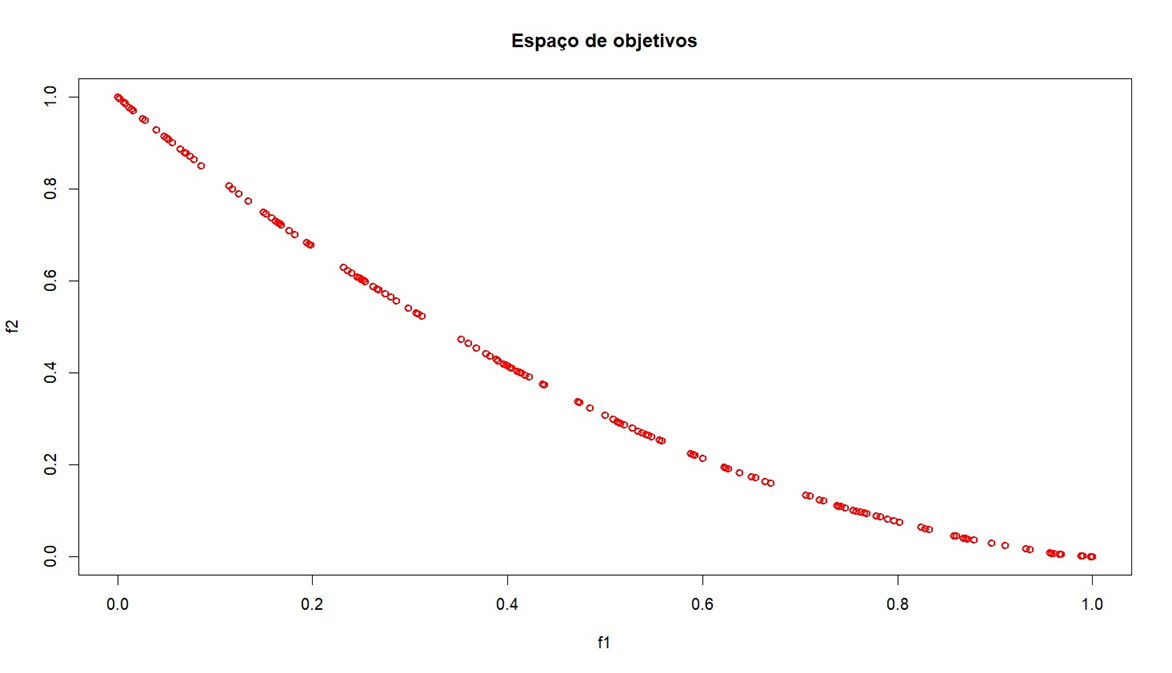
\includegraphics[width=\textwidth,trim=1 1 1 1,clip]{simplex_tc2.png}
	\end{center}
	\legend{Fonte: elaboração própria.}
\end{figure}

O objetivo agora é obter a fronteira Pareto usando o BVNS com 20 pontos
tendo como referência a 
fronteira já obtida pelo Simplex.

\chapter{Solução via BVNS}\label{cap:bnvs} 

\section{Abordagem de Soma Ponderada}

\section{Abordagem $\epsilon$-Restrito}


\chapter{Referências}\label{cap:referencias} 

\noindent M. Gendreau, J.-Y. Potvin (eds.), Handbook of Metaheuristics, Springer, 2nd ed., 2010.

\end{document}
